\documentclass{scrartcl}
\usepackage[italian]{babel}
\usepackage[utf8]{inputenc}
\usepackage{hyperref}
\usepackage{url}
\usepackage{natbib}
\usepackage{graphicx}
\usepackage{listings}
\usepackage{xcolor}
\usepackage{paralist}
\usepackage{enumitem}

\setlistdepth{9}

\newlist{myEnumerate}{enumerate}{5}
\setlist[myEnumerate,1]{label=(\arabic*)}
\setlist[myEnumerate,2]{label=(\arabic*)}
\setlist[myEnumerate,3]{label=(\arabic*)}
\setlist[myEnumerate,4]{label=(\arabic*)}
\setlist[myEnumerate,5]{label=(\arabic*)}

\definecolor{dkgreen}{rgb}{0,0.6,0}
\definecolor{gray}{rgb}{0.5,0.5,0.5}
\definecolor{mauve}{rgb}{0.58,0,0.82}

\lstdefinestyle{scalaStyle}{
  frame=tb,
  language=scala,
  aboveskip=3mm,
  belowskip=3mm,
  showstringspaces=false,
  basicstyle=\ttfamily\footnotesize,
  numbers=left,
  numberstyle=\tiny\color{gray},
  keywordstyle=\color{blue},
  commentstyle=\color{dkgreen},
  stringstyle=\color{mauve},
  frame=single,
  breaklines=true,
  breakatwhitespace=true
}

\lstset{style=scalaStyle}

\definecolor{light-gray}{gray}{0.95}
\newcommand{\code}[1]{\colorbox{light-gray}{\texttt{#1}}}
\newcommand{\emailaddr}[1]{\href{mailto:#1}{\texttt{#1}}}

\title{\LARGE
    Report finale PPS - evo-sim
}

\author{
    Rei Beshiri \\ \emailaddr{rei.beshiri@studio.unibo.it}
    \and 
    Andrea Betti \\ \emailaddr{andrea.betti10@studio.unibo.it} 
    \and 
    Daniele Giulianini \\ \emailaddr{daniele.giulianini3@studio.unibo.it}
    \and 
    Alessandro Oliva \\ \emailaddr{alessandro.oliva4@studio.unibo.it}
    \and 
    Andrea Vaienti \\ \emailaddr{andrea.vaienti2@studio.unibo.it}
}

\date{\today}

\begin{document}

\maketitle

\tableofcontents
\newpage

\section{Introduzione}
Evolution Simulator consiste nella realizzazione di un simulatore di evoluzione naturale di entità chiamate \textit{blob}, in grado di muoversi e interagire con altre entità in modalità differenti, dipendenti sia da caratteristiche generali dell'ambiente di simulazione che dalle proprietà delle entità coinvolte.

Per sopravvivere, un blob ha la necessità di mangiare cibo che gli permetta di ricaricare la sua energia vitale.

Le caratteristiche iniziali della simulazione sono parametrizzabili dall'utente attraverso un'apposita interfaccia.

Informazioni relative alle entità e agli eventi avvenuti durante la sessione verranno resi disponibili attraverso dei grafici al termine della simulazione.
\newpage

\chapter{Processo di sviluppo}
È stata adottata una metodologia di sviluppo agile che introduce un metodo di Project Management che permette di realizzare un progetto per fasi, denominate \textit{sprint}, ognuna delle quali focalizzata su nuove funzioni. Al cliente, simulato dai membri del team, viene mostrato il lavoro svolto con continuità, per verificarne il gradimento, ed è quindi possibile apportare modifiche con estrema velocità. In questo modo si incrementa l’efficienza del gruppo di lavoro e dunque la produttività.

Si è fatto riferimento a \textbf{Scrum}, scegliendo tra i membri del team Daniele Giulianini come \textbf{Product Owner} e Alessandro Oliva come \textbf{Scrum Master} ed effettuando sprint settimanali per determinare i compiti da svolgere per ciascun membro del team e rivedere le funzionalità da implementare.

Il primo periodo del processo di sviluppo è stato caratterizzato dalla modellazione dell'architettura generale del progetto, attraverso la definizione dei requisiti e una prima progettazione mediante diagrammi delle classi UML, seguito dalla creazione del \textbf{Product Backlog} e da un primo \textbf{Sprint Planning}.

\section{Meeting}
I meeting tra i componenti del team sono avvenuti con frequenza regolare mediante la piattaforma Microsoft Teams. 
I membri del team hanno partecipato attivamente agli incontri svolgendo il ruolo di sviluppatori e dove necessario quelli di Scrum Master e Product Owner.
All'inizio di ogni settimana sono stati effettuati in modo congiunto la \textbf{Sprint Review} e lo \textbf{Spint Planning}. In questo tipo di meeting è stato passato in rassegna il lavoro svolto nella settimana appena conclusa e sono stati determinati gli obiettivi e i compiti da svolgere per ciascun membro del team. Ogni componente è stato aggiornato sullo stato di avanzamento dei task individuati e il Product Backlog è stato aggiornato di conseguenza. Altri incontri si sono svolti nel mezzo della settimana per aggiornare i membri del team sui progressi svolti e far emergere problematiche riscontrate allo scopo di studiare insieme delle soluzioni, similmente a come avverrebbe nel \textbf{Daily Scrum} a cui si è fatto riferimento.

\section{Divisione dei task}
All'avvio di ciascuno sprint settimanale è stato fatto utilizzo del product backlog per assegnare a ciascun componente del team una serie di task da svolgere durante la settimana, in modo da definire obiettivi che ogni membro del team è tenuto a portare a termine. Un task rappresenta uno o più requisiti tra quelli individuati nel primo periodo del processo di sviluppo.

\section{Revisione dei task}
Alla fine di ciascuno sprint, durante la \textbf{Sprint Review}, ciascun componente del team ha informato gli altri dei progressi nello svolgimento dei task a lui assegnati, notificando le varie difficoltà avute per lo svolgimento dei task. Sulla base del risultato della review è stato aggiornato e revisionato il Product Backlog, e sono stati valutati eventuali ritardi sulla tabella di marcia adottando le relative contromisure.

Generalmente al compimento di un task, prima della sua effettiva terminazione è stata fatta un'azione di code review dove il codice prodotto dal responsabile del task è stato mostrato a tutti i membri del team con l'obiettivo di individuare possibili refactor atti a migliorare la qualità del codice prodotto, diminuendo così potenziale debito tecnico.

\section{Scelta degli strumenti}
Sono stati utilizzati differenti tool a supporto del processo di sviluppo. L'obiettivo dell'utilizzo di tali tool è quello di servire gli sviluppatori durante tutto il processo di sviluppo automatizzandolo, con lo scopo di migliorarne l'efficienza e di consentire al gruppo di concentrarsi maggiormente sulla risoluzione dei requisiti del progetto stesso.

\begin{itemize}
    \item \textbf{SBT} come strumento di build automation, automatizzando una varietà di compiti software quotidiani durante lo sviluppo del progetto come la compilazione del codice sorgente.
    \item \textbf{Scalatest} per la scrittura ed esecuzione dei test automatizzati, adottando come convenzione l'utilizzo di \texttt{FunSpec};
    \item \textbf{Travis CI} come strumento di \textbf{Continuous Integration}, in modo da testare progetti software ospitati sul repository GitHub;
    \item \textbf{GitHub} come servizio di hosting del codice sorgente e file utilizzati durente il processo di sviluppo quali ad esempio il product backlog;
    \item \textbf{FindBugs} e \textbf{Scalastyle} a supporto del controllo di qualità automatizzato del codice.
\end{itemize}
\newpage

\chapter{Requisiti}
Questo capitolo ha come scopo quello descrivere dettagliatamente tutti i requisiti del software implementato. La quasi totalità dei requisiti sono rimasti invariati sin dalle prime fasi del progetto, mentre alcuni sono stati leggermente modificati o eliminati. È bene precisare che qualunque requisito sottoelencato è stato selezionato in quanto verificabile.

\section{Requisiti di business}

L'applicazione dovrà disporre delle seguenti caratteristiche:
\begin{myEnumerate}
    \item[1] Business.
    \begin{myEnumerate}[label*=\arabic*.]
        \item[1.1] Visualizzazione di una simulazione di evoluzione naturale di entità \textit{blob} che hanno come obiettivo la sopravvivenza in un ambiente ostile;
        \item[1.2] I \textit{blob} si differenziano gli uni dagli altri in base a caratteristiche genetiche che ne influenzano il comportamento;
        \item[1.3] L'ambiente del simulatore sarà configurabile così da avere diversi scenari che influenzeranno l'andamento della simulazione.
    \end{myEnumerate}
\end{myEnumerate}

In particolare il simulatore funzionerà come segue:
\begin{itemize}
    \item Una simulazione è composta da diverse giornate in ognuna delle quali i \textit{blob} hanno l'obiettivo di procacciarsi del cibo che gli consenta di ottenere le energie necessarie a sopravvivere;
    \item I \textit{blob} per sopravvivere e riprodursi necessitano del cibo presente all'interno dell'ecosistema;
\end{itemize}

\section{Requisiti utente}
In particolare l'utente può usufruire dei seguenti aspetti:

\begin{myEnumerate}
    \item[2] Utente.
    \begin{myEnumerate}[label*=\arabic*.]
        \item[2.1] Parametrizzazione delle caratteristiche della simulazione tramite UI;
        \begin{myEnumerate}[label*=\arabic*.]
            \item[2.1.1] Cardinalità dei \textit{blob};
            \item[2.1.2] Cardinalità delle piante che producono il cibo;
            \item[2.1.3] Cardinalità massima delle giornate;
            \item[2.1.4] Cardinalità degli ostacoli presenti all'interno dell'ambiente;
            \item[2.1.5] Temperatura dell'ambiente;
            \item[2.1.6] Luminosità dell'ambiente;
        \end{myEnumerate}
        \item[2.2] Rappresentazione grafica dell'andamento della simulazione in 2D;
        \begin{myEnumerate}[label*=\arabic*.]
            \item[2.2.1] Rappresentazione delle entità all'interno dell'ambiente;
            \begin{myEnumerate}[label*=\arabic*.]
                \item[2.2.1.1] Rappresentazione dei \textit{blob};
		        \begin{myEnumerate}[label*=\arabic*.]
			        \item[2.2.1.1.2] Rappresentazione del campo visivo come circonferenza attorno al \textit{blob};
		        \end{myEnumerate}
                \item[2.2.1.2] Rappresentazione degli ostacoli;
                \item[2.2.1.3] Rappresentazione del cibo;
		\item[2.2.1.4] Rappresentazione delle piante;
            \end{myEnumerate}
            \item[2.2.2] Rappresentazione degli indicatori di evoluzione in real-time;
            \begin{myEnumerate}[label*=\arabic*.]
                \item[2.2.2.1] Rappresentazione della cardinalità della popolazione di \textit{blob} attuale;
		        \item[2.2.2.2] Rappresentazione della luminosità;
	    	    \item[2.2.2.3] Rappresentazione della temperatura;
                \item[2.2.2.4] Rappresentazione del giorno corrente;
            \end{myEnumerate}
	    \item[2.2.3] Rappresentazione dell'andamento della luminosità come indicatore cromatico sull'area della simulazione;
	    \item[2.2.4] Rappresentazione dell'andamento della temperatura come indicatore cromatico sull'area della simulazione;
        \end{myEnumerate}
	\item[2.3] Rappresentazione delle statistiche riguardanti l'andamento della simulazione;
	\begin{myEnumerate}[label*=\arabic*.]
		    \item[2.3.1] Rappresentazione della media dei valori delle caratteristiche genetiche dei \textit{blob} (velocità, percezione dell'ambiente, dimensione);
		    \item[2.3.2] Rappresentazione della cardinalità della popolazione di \textit{blob} e del cibo per ogni giornata;
		    \item[2.3.3] Rappresentazione della tipologia di entità che hanno composto la simulazione in percentuale rispetto al totale;
	    \end{myEnumerate}
	    \item[2.4] Rappresentazione della simulazione e delle statistiche finali visualizzata a schermo intero;
	    \item[2.5] Implementazione di una interfaccia testuale alternativa all'interfaccia grafica, equivalente in termini di espressività:
	    \begin{myEnumerate}
		\item[2.5.1] Lettura da console dei parametri definiti in 2.1;
		\item[2.5.2] Scrittura su console degli indicatori real-time definiti in 2.2.2;
		\item[2.5.3] Scrittura su console dei risultati della simulazione (velocità media dei \textit{blob}, dimensione media dei \textit{blob}, campo visivo medio dei \textit{blob}, numero di \textit{blob} sopravvissuti fino alla fine, quantità di cibo rimanente alla fine).
	    \end{myEnumerate}
	\end{myEnumerate}
\end{myEnumerate}

\section{Requisiti funzionali}
Il simulatore prodotto dovrà:

\begin{myEnumerate}
    \item[3] Funzionali.
    \begin{myEnumerate}[label*=\arabic*.]
	\item[3.1] Essere composto da giornate che si compongono di un numero fisso di iterazioni le quali sono l'unità temporale di aggiornamento della simulazione;
        \item[3.2] Supportare diverse tipologie di entità;
	\begin{myEnumerate}[label*=\arabic*.]
        	\item[3.2.1] \textit{blob};
		\begin{myEnumerate}[label*=\arabic*.]
        		\item[3.2.1.1] I \textit{blob} hanno delle caratteristiche genetiche di base;
			\begin{myEnumerate}[label*=\arabic*.]
        			\item[3.2.1.1.1] Velocità;
				\item[3.2.1.1.2] Campo visivo circolare;
				\item[3.2.1.1.3] Dimensione;
				\item[3.2.1.1.4] Vita;
    			\end{myEnumerate}
			\item[3.2.1.2] Possibilità per i \textit{blob} di disporre di abilità aggiuntive;
			\begin{myEnumerate}[label*=\arabic*.]
        			\item[3.2.1.2.1] Cannibalismo che implica la possibilità di nutrirsi di altri blob di dimensione inferiore alla propria per incrementare la vita;
				\item[3.2.1.2.2] Avvelenamento che implica una perdita maggiore di vita con l'avanzamento del tempo;
				\item[3.2.1.2.3] Rallentamento che implica una diminuzione della velocità di movimento;
    			\end{myEnumerate}
    		\end{myEnumerate}
		\item[3.2.2] Cibi il cui consumo provoca diversi effetti sui \textit{blob}
		\begin{myEnumerate}[label*=\arabic*.]
        		\item[3.2.2.1] Nutriente che implica l'aumento di vita attuale del \textit{blob};
			\item[3.2.2.2] Avvelenato che implica l'applicazione dello stato di rallentamento sul blob che vi collide;
			\item[3.2.2.3] Riproduttivo che implica la nascita di un nuovo blob, e un aumento della vita attuale del padre;
			\begin{myEnumerate}[label*=\arabic*.]
        			\item[3.2.2.3.1] Possibilità che un blob sia cannibale alla nascita;
    			\end{myEnumerate}
    		\end{myEnumerate}
		\item[3.2.3] Ostacoli la cui collisione impedisce il naturale movimento del \textit{blob};
		\begin{myEnumerate}[label*=\arabic*.]
        		\item[3.2.3.1] Dannoso che implica il decremento della vita del blob che vi collide;
			\item[3.2.3.2] Rallentatore di movimento che implica l'applicazione dello stato di rallentamento sul blob che vi collide;
    		\end{myEnumerate}
    	\end{myEnumerate}
	\item[3.3] Parametrizzazione delle diverse caratteristiche ambientali che influenzano tutti i \textit{blob};
	\begin{myEnumerate}[label*=\arabic*.]
        	\item[3.3.1] Temperatura che influenza la velocità di movimento;
		\item[3.3.2] Luminosità che influenza la percezione dell'ambiente;
    	\end{myEnumerate}
	\item[3.4] Movimento dei \textit{blob} all'interno dell'ambiente dettato da un AI;
	\begin{myEnumerate}[label*=\arabic*.]
        	\item[3.4.1] Movimento casuale finché non compare un entità commestibile all'interno del campo visivo;
		\item[3.4.2] Inseguimento dell'entità commestibile presente all'interno del campo visivo;
    	\end{myEnumerate}
	\item[3.5] Riproduzione dei \textit{blob} basata sulle caratteristiche genetiche del padre con una variazione randomica;
	\item[3.6] Possibilità di effettuare simulazioni con la possibilità per l'utente di specificare le caratteristiche della simulazione come descritto in 2.1;
	\item[3.7] Possibilità di visualizzare l'andamento della simulazione;	
	\begin{myEnumerate}[label*=\arabic*.]
		\item[3.7.1] Visualizzazione delle entità all'interno dell'ambiente come descritto in 2.2.1;
		\item[3.7.2] Visualizzazione degli indicatori di evoluzione in real-time come descritto in 2.2.2;
	\end{myEnumerate}
	\item[3.8] Possibilità di visualizzare i risultati finali della simulazione attraverso grafici;
	\end{myEnumerate}
\end{myEnumerate}

\section{Requisiti non funzionali}

\begin{myEnumerate}[label*=\arabic*.]
	\item[4] Non funzionali
	\begin{myEnumerate}[label*=\arabic*.]
		\label{sec:cpu}
		\item[4.1] Mantenimento di un framerate stabile e costante che si aggiri sui 60 FPS su una macchina con requisiti minimi di 4GB di RAM, CPU Dual Core da 2.8 GHz.
		\item[4.2] Interfaccia utente responsive;
	\end{myEnumerate}
\end{myEnumerate}


\section{Requisiti di implementazione}

\begin{myEnumerate}[label*=\arabic*.]
	\item[5] Implementazione
	\begin{myEnumerate}[label*=\arabic*.]
		\item[5.1] L'applicazione verrà sviluppata in Scala e Prolog, mentre per verificare la presenza di errori verranno implementati test in Scalatest.
	\end{myEnumerate}
\end{myEnumerate}
\newpage

\section{Analisi del Dominio}

Il progetto ha lo scopo di simulare il ciclo di vita di creature virtuali denominate \textit{blob} e immerse in un ambiente virtuale 2D dotato di fonti di cibo ed ostacoli.
Prima di ogni simulazione sarà possibile tramite un'apposita UI permettere la parametrizzazione di diverse caratteristiche del mondo simulato da parte dell'utente.
Le caratteristiche ambientali che possono essere parametrizzate sono:
\begin{itemize}
    \item numero di entità Blob presenti nella simulazione. I blob generati all'inizio della simulazione si dividono in:
    \begin{enumerate}
        \item Base Blob;
        \item Cannibal Blob.
    \end{enumerate}
    \item numero di entità Plant presenti all'interno della simulazione. I tipi di piante si suddividono in:
    \begin{enumerate}
        \item Standard Plant;
        \item Reproducing Plant;
        \item Poisonous Plant.
    \end{enumerate}
    \item numero di entità Obstacle presenti all'interno della simulazione;
    \item la luminosità all'interno del mondo simulato;
    \item la temperatura all'interno del mondo simulato;
    \item la durata in giorni della simulazione.
\end{itemize}

Una volta avviata la simulazione verranno disposte le entità all'interno del mondo, e i blob inizieranno quindi a muoversi in cerca di cibo, cercando di non morire in quanto la loro vita si riduce nel tempo. 

Un blob può avere diversi valori di dimensione, velocità e ampiezza del campo visivo, che definiscono il progresso della simulazione.

Vi sono presenti diverse tipologie di blob:
\begin{itemize}
    \item Base Blob: blob standard il quale obiettivo è quello di sopravvivere il più a lungo possibile, consumando il cibo che trova all'interno del mondo. Si muoverà in direzione del cibo più vicino nel caso sia all'interno del suo campo visivo;
    \item Cannibal Blob: diversamente dal Base Blob questo tipo di blob può nutrirsi di cibo e degli altri Base Blob, se questi ultimi hanno una dimensione minore;
    \item Poison Blob: il Poison Blob è una tipologia di blob con un effetto temporaneo applicato da un cibo velenoso. La sua vita si riduce in maniera più rapida per un certo periodo di tempo;
    \item Slow Blob: lo Slow Blob è una tipologia di blob con un effetto temporaneo applicato da un ostacolo. La sua velocità è ridotta per un certo periodo di tempo.
\end{itemize}

Il cibo viene prodotto ciclicamente da un pianta, ogni pianta produce una certa tipologia di cibo, ed ogni cibo può avere diversi \textit{effetti} sui blob:
\begin{itemize}
    \item Standard Effect: il cibo incrementa la vita del blob che lo ha mangiato;
    \item Poisonous Effect: il cibo avvelena il blob facendolo diventare un PoisonBlob;
    \item Reproduce Effect: il cibo permette al blob di riprodursi creando un Blob figlio differente dal padre.
\end{itemize}
Dopo un determinato numero di iterazioni a partire dalla sua generazione o alla collisione con un blob, il cibo viene rimosso dal mondo.

Il blob prima di muoversi verso un cibo deve prima poterlo vedere nel suo campo visivo. Il campo visivo di un blob dipende da un valore iniziale e dalla luminosità che varia durante le fasi di un giorno. Intuitivamente quando è più luminoso i blob potranno vedere ad una distanza maggiore rispetto a quando la luminosità si abbassa.

Così come la luminosità anche la temperatura ha un'effetto attivo sui blob, che anch'essa varia durante l'arco della giornata influenzando la velocità di un blob.

Un blob muovendosi può incorrere in un ostacolo, e ogni ostacolo ha un effetto diverso:
\begin{enumerate}
    \item Slow Effect: l'ostacolo rallenta il blob facendolo diventare Slow Blob;
    \item Damage Effect: l'ostacolo danneggia il blob causandogli danno.
\end{enumerate}
\newpage

\section{Design Architetturale}

\subsection{Architettura generale}



Per garantire una corretta separazione delle responsabilità fra componenti, il progetto adotta il pattern architetturale MVC in modo da mantenere l’intera architettura il quanto più possibile modulare e flessibile.

In particolare dovendo fornire all'utente diverse interfaccie grafiche per interagire e monitorare la simulazione, si è deciso di utilizzare tale pattern in modo da mantenere l’intera architettura quanto più modulare e flessibile possibile.

\begin{figure}[h!]
\centering
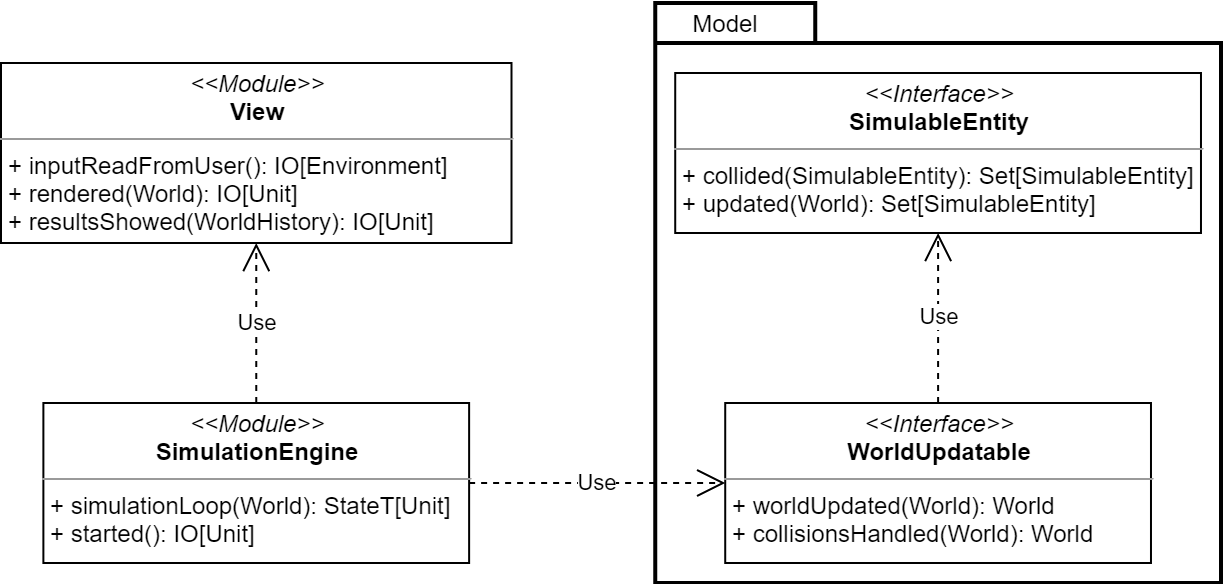
\includegraphics[width=\textwidth, scale=0.44]{img/MainArchitecture.png}
\caption{Design architettura principale}
\label{fig:mainarchitecture}
\end{figure}

\subsection{Pattern MVC}
Come mostrato in Figura \ref{fig:mainarchitecture} le componenti sono interamente indipendenti tra di loro, permettendo una buona separazione delle responsabilità fra le stesse.

\begin{itemize}
    \item Il model interpreta il comportamento dell’applicazione in termini di dominio del problema, in maniera del tutto indipendente dall’interfaccia utente. Il modello gestisce quindi i dati, la logica e le regole dell’applicazione.
    \item Il controller si occupa principalmente di eseguire ed applicare la logica di gioco e di aspetti di interazione tra model e view.
    \item La view visualizza i dati contenuti nel model secondo una rappresentazione testuale o grafica e si occupa dell'interazione tra il simulatore e gli utenti.
\end{itemize}

La separazione dei compiti e dei componenti proposta dall'approccio MVC favorisce il riuso del codice, un aumento della produttività, facilita la manutenzione del software e ne agevola la scalabilità. Nello specifico i vantaggi sono i seguenti:
\begin{itemize}
    \item Esiste la possibilità di scrivere view e controller diversi, utilizzando lo stesso model e quindi, come già accennato, riutilizzare parte del codice scritto in precedenza.
    \item L'utilizzo di un modello rigido e di regole standard nella stesura del progetto facilita un eventuale lavoro di manutenzione e agevola la comprensione anche da parte di altri programmatori esterni.
    \item La possibilità di avere un controllore separato dal resto dell’applicazione, rende la progettazione più semplice e permette di concentrare gli sforzi sulla logica del funzionamento.
    \item Un cambiamento ad un componente generalmente non comporta alcuna modifica necessaria agli altri componenti.
\end{itemize}

\newpage

\chapter{Design di dettaglio}

Dopo aver descritto l’architettura del sistema si procede con il design di dettaglio delle sue componenti principali. 
L’approccio progettuale utilizzato combina aspetti Object-oriented, come l’utilizzo dell’interfaccia come astrazione attraverso la quale caratterizzare i componenti, per scatenare comportamenti diversi su entità soggette ad un comune contratto, con elementi di programmazione funzionale pura, quali la tendenza all’impiego di strutture dati immutabili e la riduzione di side effects, favorendo la descrizione lazy della computazione, la separazione fra componente strutturale e comportamentale delle entità ed altri elencati di seguito.


\section{Core}

\section{SimulationEngine e monadi}
Il motore della simulazione \code{SimulationEngine} consiste in una descrizione monadica delle fasi della simulazione, che prevede l’aggiornamento dei parametri del mondo, il rilevamento e risoluzione delle collisioni fra le entità che lo popolano, la visualizzazione a video del suo stato aggiornato e l’attesa dell’intervallo di tempo prima della successiva iterazione. In questo modo il codice non contiene i side-effect invece presenti in un’equivalente versione procedurale, e la parte non funzionalmente pura è confinata, per quel che riguarda il core, all’avvio della applicazione. 
Questo andamento sequenziale e periodico è stato modellato attraverso una composizione di state monad \code{State[World, A]} (per quanto riguarda l’aggiornamento della struttura del mondo) e di IO monad (per le operazioni di I/O come il display a video delle entità e delle statistiche storiche alla chiusura dell’applicazione). Per tale motivo (e a fini di leggibilità) sono stati definiti i type alias: type SimulationIO[A] = IO[A] e type Simulation[A] = StateT[SimulationIO, World, A]


\begin{verbatim}
MISSING SNIPPET
\end{verbatim}

La IO monad permette di esprimere una computazione in modo lazy, e in più, la state monad consente di rendere implicito il passaggio di stato aggiornato fra le operazioni sequenziali di manipolazione del mondo, ciascuna delle quali determina una sua nuova versione. Al fine di combinare 2 monadi differenti, che in quanto tali non si possono comporre fra di loro\footnote{Rúnar Bjarnason and Paul Chiusano. Functional Programming in Scala. Exercise 12.11.}, è stato utilizzato il monad transformer \code{StateT: (StateT[SimulationIO, World, A])}.

\section{Queriable type class e ad-hoc polimorphism}
Di supporto alla gestione delle collisioni è definita la typeclass Queriable, che permette ad un type functor di acquisire la capacità di essere interrogabile sulla presenza di un dato elemento al suo interno. La disponibilità in scope di una conversione implicita da qualsiasi funtore di un tipo generico a Queriable gli permette non solo di verificare se un elemento di tale tipo generico è da esso contenuto, ma di abilitare una serie di algoritmi già implementati e riusabili (fra i quali containedAnyOf e containedAllOf). La possibilità di abilitare a posteriori tali conversioni implicite rende questa astrazione (e l’insieme degli algoritmi che la sfruttano) applicabile retroattivamente a tipi già esistenti, oltre che a quelli futuri, offrendo un meccanismo di ereditarietà più flessibile dell’ereditarietà. Per implementare la type class, che in scala non è attualmente disponibile come astrazione di prima classe, e attivare il meccanismo di conversione implicita sono stati sfruttati gli higher-kinded-type assieme ai context-bound.

\section{Model}

\subsection{Struttura entità con mixin}
Per la modellazione degli aspetti strutturali delle entità del \code{World} si è sfruttato il meccanismo dei self-type al fine di rendere modulare l’acquisizione di ogni singola caratteristica genetica della popolazione attraverso l’algoritmo di linearizzazione predisposto da scala. Una volta definiti, con un’ottica molto granulare, un set di proprietà e i self-type corrispondenti, attribuendo a ciascuno di essi un dominio minimale ed una singola proprietà/funzionalità, la definizione della componente strutturale delle entità richieste dai requisiti si riduce ad un’attività di composizione di moduli elementari. Ciò porta ad una struttura composta da più livelli di componenti, alcuni dei quali condivisi da più entità. Questo approccio rende riutilizzabili in futuro le astrazioni già definite permettendo di combinare i diversi tratti genetici con flessibilità.

\begin{figure}[h!]
\centering
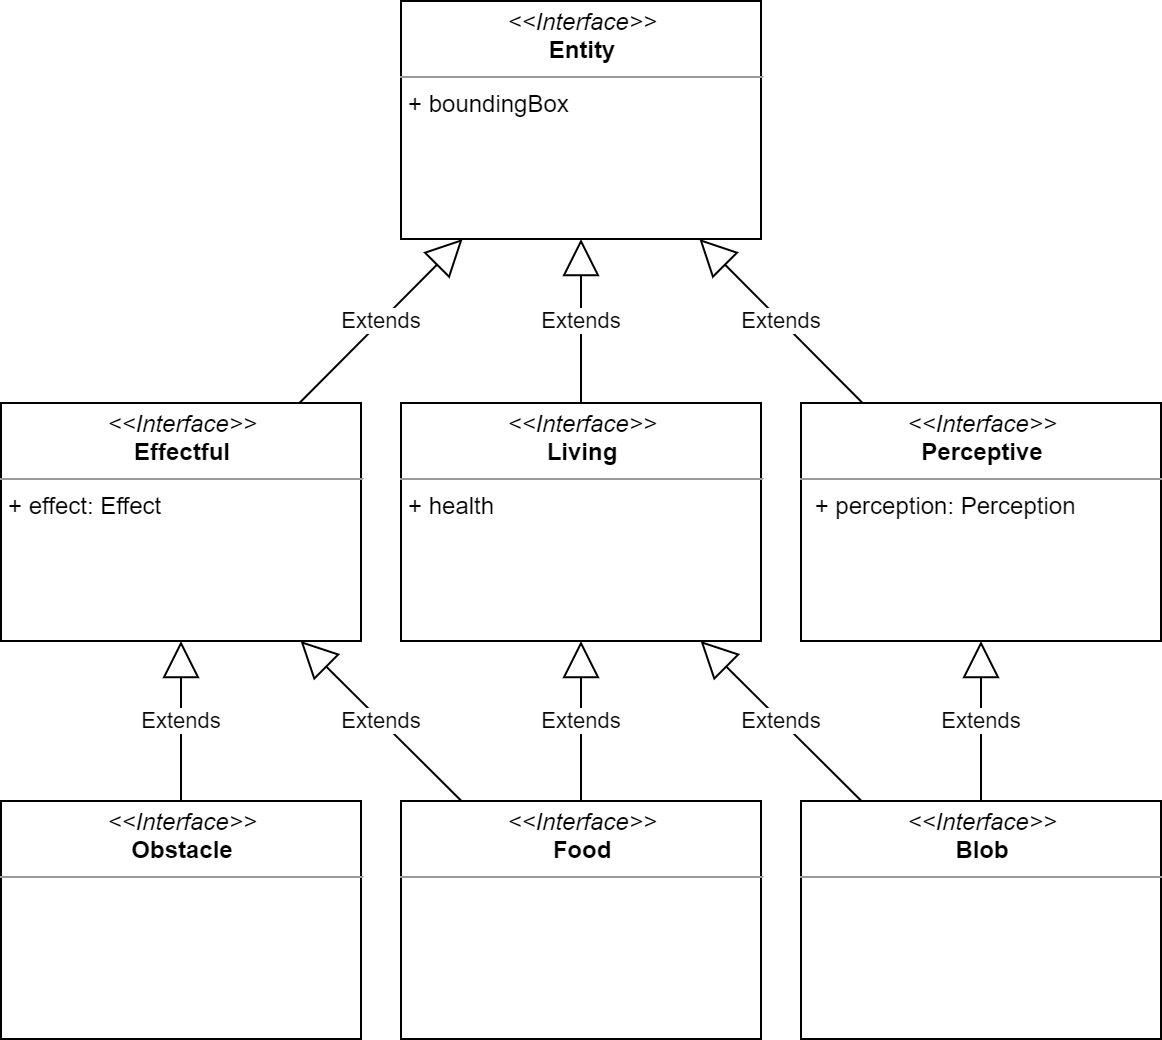
\includegraphics[width=\textwidth, scale=0.44]{img/ModelHierarchy.png}
\caption{Dettaglio UML sulla gerarchia strutturale delle entità della simulazione. Ciascun astrazione identifica una singola funzionalità.}
\label{fig:modelhierarchy3}
\end{figure}

Come proprietà della struttura sono utilizzati diversi parametri higher order (come \code{MovementStrategy}, \code{DegradationEffect} e \code{CollisionEffect}), che fungono da strategie e definiscono il comportamento dell’entità per aspetti specifici (la degradazione della propria vita o il movimento all’interno dell’area di simulazione, ad esempio). Ciò permette di riutilizzare una stessa struttura per modellare una serie di comportamenti diversi, piuttosto che codificare tale diversità di comportamento nel codice, trasferendola dunque a livello di istanza anziché di classificazione (dall’aspetto intensionale a quello estensionale). Invece di esprimere nel codice di una entità la logica di alcuni aspetti specifici, si incapsula dunque tale gestione in un parametro higher order, permettendo ad esempio di riutilizzare anche per entità con diverse logiche di degradazione la struttura rimanente. Al contempo, chiunque vorrà estendere il sistema di simulazione in futuro potrà usufruire di tali strategie per l’implementazione delle sue componenti.

\subsection{Comportamento entità con self type}
L’aspetto comportamentale delle entità, che riguarda cioè le operazioni che agiscono sul loro stato in occasione dell’evento di aggiornamento del mondo e di collisione con altre entità, è gestito mediante 2 trait con self types: \code{Updatable} e \code{Collidable}. Questa modellazione prevede di sfruttare la interfaccia per variare il comportamento sotto la stessa astrazione e fornire estendibilità futura e, al contempo, un approccio funzionale nella gestione dello stato (ogni entità è immutabile e l’aggiornamento coincide con la generazione di una nuova versione con proprietà modificate). Le signature di \code{Updatable} e \code{Collidable} prevedono di restituire un set di \code{SimulableEntity} che rimpiazza l’entità nell’iterazione successiva e permette di esprimerne la rimozione, l’aggiornamento o eventi quali la riproduzione o la clonazione della stessa.

\begin{figure}[h!]
\centering
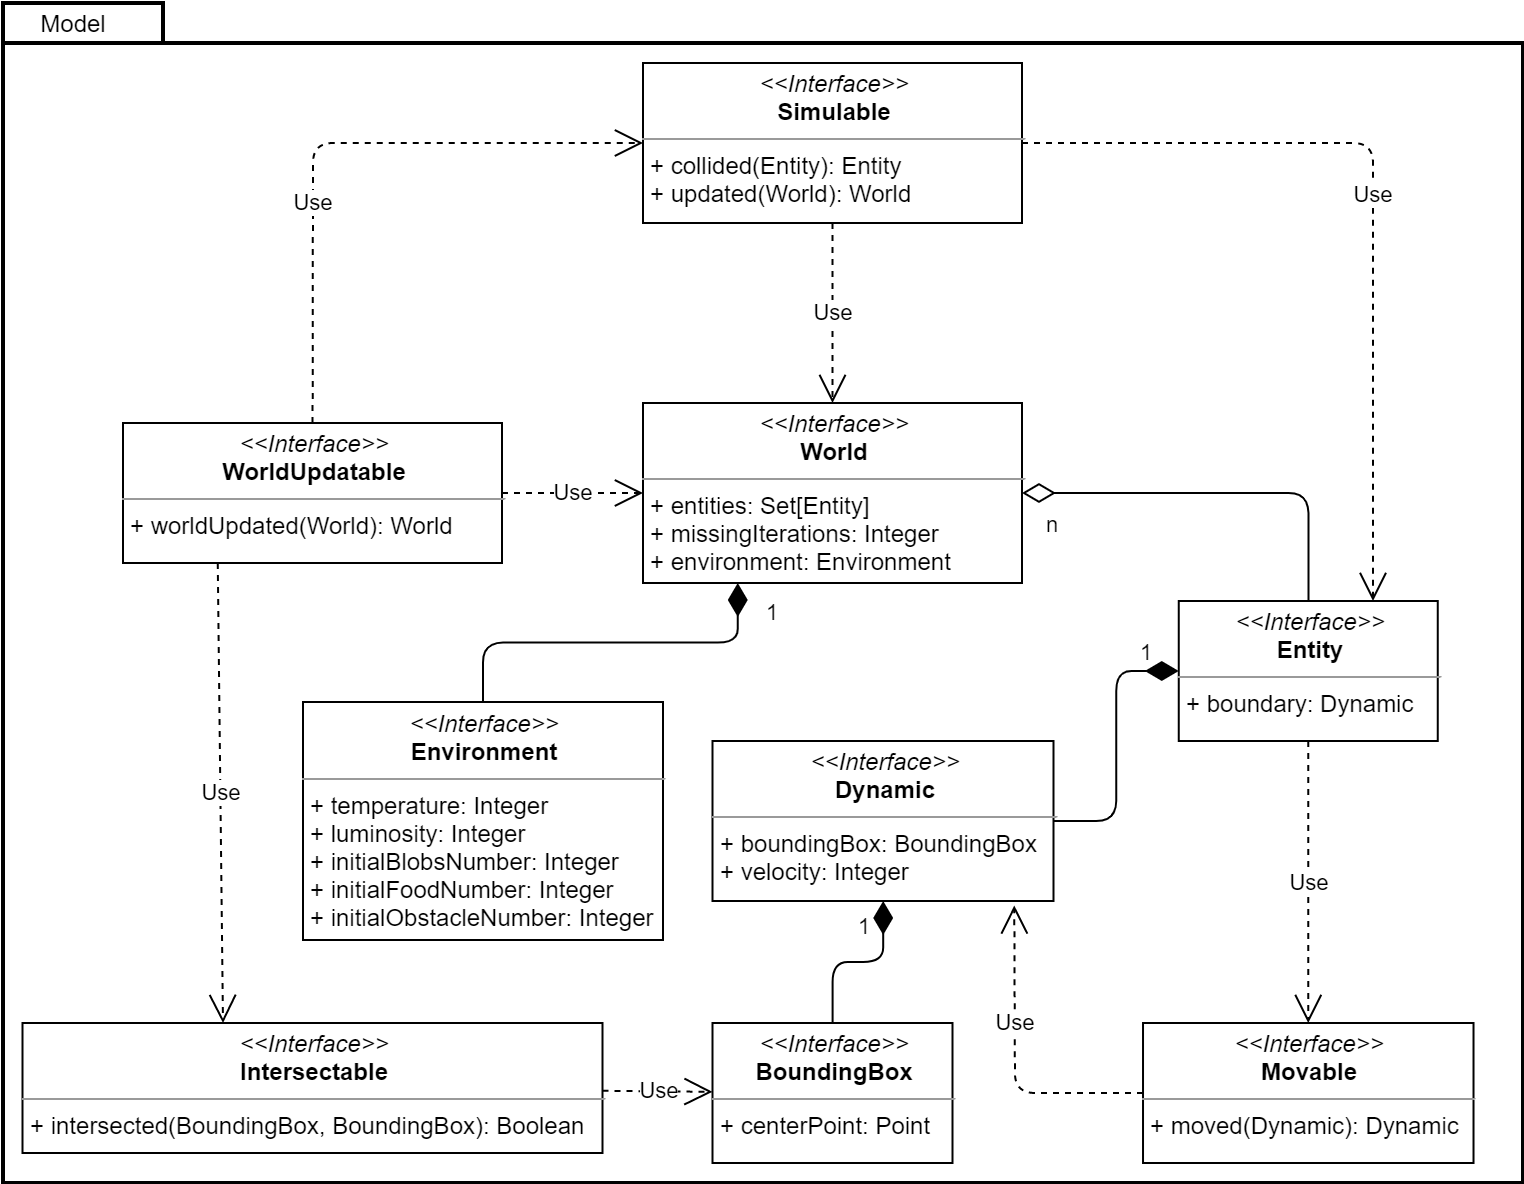
\includegraphics[width=\textwidth, scale=0.14]{img/Model.png}
\caption{Dettaglio UML complessivo degli aspetti comportamentali della entità e della simulazione e della integrazione con il core. }
\label{fig:model}
\end{figure}

Il requisito che un’entità deve soddisfare per partecipare ad una simulazione si suddivide in 2 componenti, rappresentati dal type alias \code{SimulableEntity}: dal punto di vista strutturale il vincolo di rappresentare una Entity, mentre, dal punto di vista comportamentale, quello di disporre di un’implementazione di tali 2 trait, la cui unione è definita mediante il type alias \code{Simulable}.

\begin{verbatim}
MISSING SNIPPET
\end{verbatim}

A tale scopo, i companion object di \code{Updatable} e \code{Collidable} forniscono delle implementazioni dei rispettivi trait pronte all’uso per comportamenti riusabili e applicabili intercambiabilmente a qualunque Entity. (\code{NeutralUpdatable} e \code{NeutralCollidable} definiscono dei comportamenti che decorano i tipi sottostanti non inducendo nessuna modifica nella entità su cui vengono installati). Per questo motivo, in ottica futura, l’implementazione di Entity è sufficiente a disporre di nuove entità potenzialmente integrabili all’interno della simulazione.

\section{View}

Le operazioni di input e output della view consistono in descrizioni monadiche lazy della costruzione e comportamento dei componenti, così da aderire al paradigma funzionale nonostante la tipica natura object-oriented dei componenti di View. Sono state individuate un'operazione di input e due di output. La prima consiste nella lettura dei parametri di inizializzazione della simulazione contenuti in un oggetto \code{Environment} che verrà usato per la costruzione del \code{World}. La prima operazione di output viene richiamata ad ogni iterazione e fornisce lo stato attuale del \code{World} e delle entità che lo popolano. L'ultima, dato lo storico di tutte le istanze di \code{World} in modo lazy, provvede all'aggregazione delle informazioni contenute per fornire statistiche sulla simulazione.


\newpage

\section{Implementazione}
Il seguente capitolo motiva e dettaglia le scelte implementative ritenute rilevanti per una corretta comprensione del progetto. È bene precisare che nel codice è presente la Scaladoc che permette di dettagliare ogni singola parte del codice.


\subsection{Paradigma funzionale}
Sin dalle prime fasi di progettazione il team ha intrapreso la scelta di utilizzare il più possibile il paradigma funzionale, cercando di non ricorrere alle usuali abitudini di programmazione object-oriented. Per fare ciò sono stati utilizzati diversi criteri: 
\begin{itemize}
    \item inutilizzo dei side effect, creando ad ogni modifica un nuovo ogetto immutabile.
    \item utilizzo di funzioni ricorsive.
    \item utilizzo di funzioni higher-order che permettono una facile ed immediata realizzazione del parttern Strategy, consentono una maggiore riutilizzabilità del codice. In questo modo è possibile passare alle funzioni strategie esterne, non necessitando così di modificare il codice.
\end{itemize}

Rispettando quanto sopra elencato, il Controller e il Model dell'applicazione sono stati realizzati con un approccio puramente funzionale. La View adottare anch'essa il paradigma descritto in questo corso attraverso l'utilizzo della libreria cats.effect.IO.

\subsubsection{View}
Bisogna parlare della View, in particolare dell'approccio funzionale utilizzato.


\subsubsection{Monadi}


\subsubsection{World e Stream}
Il World è stato modellato come un contenitore immutabile delle proprietà della simulazione e delle entità che vi partecipano. Al fine di memorizzare i dati necessari ai fini di analisi, esso è definito in termini di se stesso: la worldHistory è uno stream costituito dalle istanze di World riferite alle iterazioni precedenti. La lazy evaluation degli stream permette di non appesantire la computazione del simulationLoop con un carico di lavoro altrimenti insostenibile: impiegare una collezione non lazy come una lista avrebbe comportato la creazione di una moltitudine di strutture dati intermedie di grandissime dimensioni. 

\begin{figure}[h!]
\centering
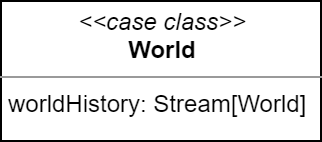
\includegraphics[scale=0.30]{img/WorldDetail.png}
\caption{Dettaglio di worldHistory come Stream per la memorizzazione delle informazioni sugli World alle iterazioni passate necessarie alla elaborazione statistica finale}
\label{fig:worldDetail}
\end{figure}

Grazie agli stream, la valutazione della grande quantità di dati accumulata avviene solo alla conclusione della simulazione e al momento del processamento dei dati a fini statistici, non interferendo così con l’andamento della simulazione.

\subsubsection{Currying e partial application}


\subsubsection{Memoizing}

\subsection{Paradigma logico}
Dopo un accurata e dettagliata analisi della logica di movimento delle entità, il team si era proposto di integrare nel progetto il paradigma logico. Ciò è avvenuto attraverso la libreria TuProlog. In particolare, la logica di movimento ideata e implementata è la seguente:
\begin{itemize}
    \item nel caso in cui nessuna entità commestibile sia presente all'interno del campo visivo, l'entità in considerazione deve muoversi in una direzione casuale.
    \item nel caso in cui una o più entità commestibili siano presenti all'interno del campo visivo, l'entità dovrà dirigersi verso il nutrimento più vicino.
\end{itemize}
La teoria Prolog presente nel file \code{src/main/resources/movementTheory.pl} consente di ricercare la presenza di un entità commestibile all'interno del campo visivo tra tutte le entità presenti nella simulazione, ed agire di conseguenza nel caso in cui l'entità sia presente o meno all'interno del campo visivo. Tuttavia per problemi legati alle performance (in quanto non possibile rispettare il requisito 4.1) si è adottato un approccio ibrido, in cui la ricerca di un entità all'interno del campo visivo viene effettuata con il paradigma funzionale, lasciando poi il calcolo della nuova posizione al paradigma logico.

\subsection{Test}
La realizzazione di test è stato un aspetto fondamentale per verificare la correttezza e la qualità del codice, garantendo anche un'ulteriore documentazione del software sviluppato. La loro implementazione non è avvenuta con la metodologia stringente del Test Driven Development (TDD), bensì con un approccio più tradizionale, in cui la funzionalità veniva testata una volta pronta. In particolare è stata utilizzata la libreria ScalaTest, mantenendo uno stile omogeneo utilizzando \textbf{FunSpec}.

\subsection{Suddivisione del lavoro}
Inizialmente il team ha effettuato un analisi preliminare, dettagliando quali caratteristiche e requisti il software dovesse esibire. In seguito a ciò, si sono susseguiti una frequente serie di meeting (in cui era presente tutto il team) dove, partendo da piccoli diagrammi UML che descrivevano a grandi linee l'architettura del sistema, si è scesi sempre più in dettaglio fino a creare l'intero design architetturale. È bene precisare che il design architetturale è stato ideato in ciascuna sua parte da tutto il team, in modo coeso e collaborativo. Successivamente, in seguito alla realizzazione di un design architetturale dettagliato per ogni funzionalità del software, a ciascun membro del team è stata assegnata una parte dello sviluppo. Nel dettaglio:

\subsubsection{Rei Beshiri}
Il mio ruolo nel progetto dal punto di vista implementativo riguarda principalmente lo sviluppo del model e delle sue diverse componenti in collaborazione con i membri del team, in particolare delle entità \textit{blob} del loro comportamento e reazione all'ambiente circostante e alle intersezioni tra le varie entità in gioco e degli effetti delle stesse così come della loro bounding box.

I test sviluppati riguardano le classi \code{BlobTest}, \code{DegradationTest}, \code{IntersectionTest}.

\subsubsection{Andrea Betti}
Ho contribuito insieme a Rei Beshiri all'implementazione dei comportamenti delle diverse entità della simulazione in \code{evo\_sim.model.EntityBehaviour} e agli effetti applicabili dalle entità \textit{Effectful} in \code{evo\_sim.model.effects.CollisionEffect}, realizzando le classi e le funzioni relative alle entità \textit{Food} e \textit{Plant} e contribuendo in misura minore ai comportamenti delle entità \textit{Blob} e all'estensione di \code{evo\_sim.model.EntityStructure}.

Ho inoltre implementato la logica di rappresentazione della simulazione utilizzando \texttt{scala-swing} all'interno della classe \code{evo\_sim.view.swing.custom.components.ShapesPanel}, utilizzata nella funzione \code{rendered} di \code{evo\_sim.view.swing.SwingView} realizzata da Alessandro Oliva.

Per quanto riguarda i test, ho realizzato \code{FoodTests} e \code{PlantTests}.

\subsubsection{Daniele Giulianini}

\subsubsection{Alessandro Oliva}
Il mio contributo nel model è consistito nello sviluppo delle entità \textit{Obstacle}, le entità con status temporanei (il cui raffinamento è però stato curato da Rei Beshiri), in particolare lo \textit{SlowBlob}.

Mi sono occupato inoltre del ciclo giorno notte della simulazione, con rispettiva influenza sui blob in termini di velocità e campo visivo tramite appositi moduli di funzioni.

Per quanto riguarda la View, ne ho seguito lo sviluppo dalla prima versione in \texttt{ScalaFX} fino all'implementazione puramente funzionale attraverso il framework \texttt{Cats}, del quale con l'importante contributo di Daniele Giulianini è stato sviluppato un intero package che permette di utilizzare componenti Swing in maniera funzionale. Sempre con Daniele Giulianini mi sono occupato dell'integrazione fra View e Core mediante il framework monadico. Parallelamente a questa versione è stata sviluppata un interfaccia a linea di comando per permettere la fruizione dell'applicazione nella sua interezza anche mentre si lavorava alla View.

I test da me sviluppati sono inclusi in \code{ObstacleTests}.
\subsubsection{Andrea Vaienti}
\newpage

\section{Retrospettiva}

\subsection{Avviamento}
La fase di avviamento si è incentrata sulla definizione dei requisiti di base del progetto, analisi del problema e definizione dei componenti principali del sistema. Queste operazioni hanno portato via molto tempo ma ci ha permesso di avere le idee chiare fin da subito, così da evitare di tornare sui propri passi per via di questioni definite in modo troppo opaco o generico. Buona parte della stesura della documentazione è stata prodotta in questa fase, così da consolidare termini, comportamento della simulazione e definire la struttura del sistema ad un grado sufficientemente fine di granulatirà. Sono stati anche preparati i tool di sviluppo, in particolare \textbf{SBT} e \textbf{Travis CI}.
\newpage

\end{document}